\chapter{Nuevos ejercicios con físicas realistas}
\label{chap:nuevos_ejercicios} 
En este capítulo se presentan los nuevos ejercicios que se han creado para enriquecer el contenido ofrecido en el entorno de \textit{Kibotics}. Todos ellos permiten explotar las mejoras que ofrece el motor de físicas complementario implementado.

\section{Sigue-líneas con rampa}
Este ejercicio\footnote{\url{https://www.youtube.com/watch?v=PjTr13M3o5k}} se basa en la propuesta realizada para la competición \textit{Robocup Junior Australia 2019}\footnote{https://www.robocupjunior.org.au/}. Se trata de una versión mejorada del sigue-líneas tradicional, en el que se incluyen trayectorias más complejas y diversas y dos niveles diferentes conectados a través de una rampa. Actualmente, este ejercicio está disponible en la plataforma \textit{Kibotics} como un ejercicio a resolver en \textit{Python o Scratch} y el robot que se ha seleccionado para su solución ha sido el mBot.  

\newpage

\begin{figure}[h!]
    \centering
    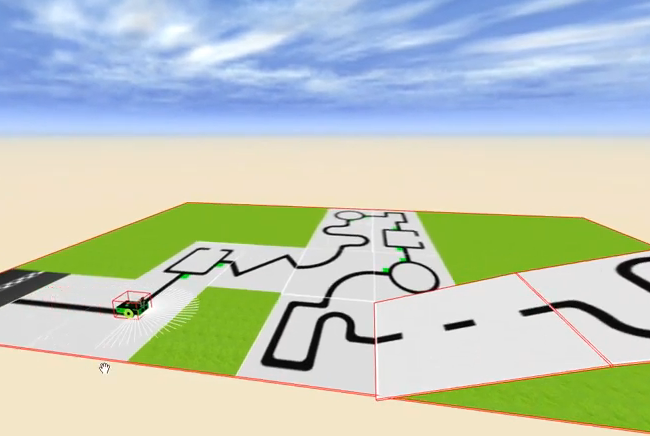
\includegraphics[width=0.8\textwidth, height=0.8\textwidth]{siguelineas.png}
    \caption{Escenario Sigue-líneas con rampa}
    \label{fig:Sigue-líneas con rampa 2}
\end{figure}

El ejercicio  aprovecha las ventajas del motor de físicas complementario en la subida de las rampas. Durante la subida, \textit{CANNON} materizaliza la fricción oponiendo fuerzas de rozamiento al movimiento, mientras que el motor complementario se encarga de aplicar la fuerza autónoma necesaria para lograr que el robot ascienda por la rampa. La fuerza resultante será más grande que la necesaria para avanzar por el suelo plano sin inclinación y, además, será necesario tener en cuenta el valor de la fricción y la inclinación de la rampa para hacer más fácil o difícil la subida. Tal y como ocurriría en la realidad con un robot físico, se alcanzará un grado de inclinación o un valor de fricción con los cuales el mBot no será capaz de avanzar por la rampa puesto que el diseño del motor incluye un límite de fuerza máxima aplicable\footnote{\url{https://www.youtube.com/watch?v=8mtK8DVkDZo}}.


\begin{figure}[h!]
\begin{subfigure}[b]{0.5\textwidth}
    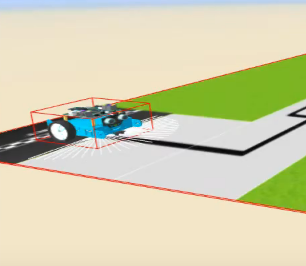
\includegraphics[width=\textwidth, height=\textwidth]{rampa_ej0.png}
  \end{subfigure}
  \hfill
  \hfill
  \begin{subfigure}[b]{0.5\textwidth}
    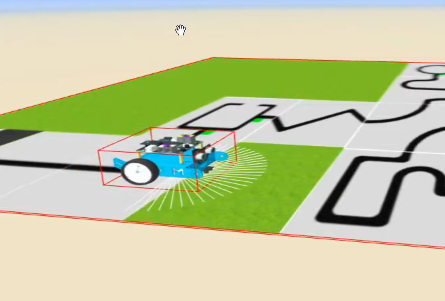
\includegraphics[width=\textwidth, height=\textwidth]{rampa_ej.png}
  \end{subfigure}
    \hfill
    \hfill
  \begin{subfigure}[b]{0.5\textwidth}
    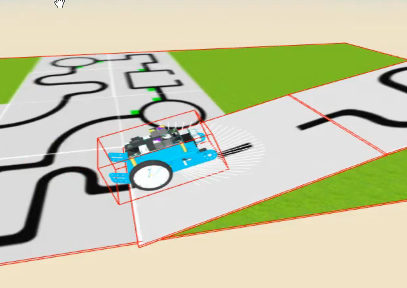
\includegraphics[width=\textwidth, height=\textwidth]{rampa_ej2.png}
  \end{subfigure}
    \hfill
  \begin{subfigure}[b]{0.5\textwidth}
    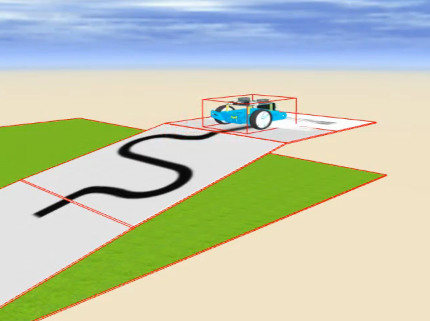
\includegraphics[width=\textwidth, height=\textwidth]{rampa_ej3.png}
  \end{subfigure}
    \caption{Fotograma del movimiento del ejercicio Sigue-líneas con rampa}
    \label{fig:Sigue-líneas con rampa}
\end{figure}

\clearpage

A continuación, en la tabla \ref{tabla:param_ej1}, se recoge el valor de los parámetros del modelo de fuerzas y de  \textit{A-Frame} necesarios para el correcto funcionamiento del motor de físicas complementario y que caracterizan este ejercicio.

\begin{table}[h!]
\centering
\begin{tabular}{|c|c|}
\hline
\multicolumn{2}{|c|}{\textbf{Parámetros del modelo de fuerzas}}                \\ \hline
mass                                           & 1                             \\ \hline
inertia                                        & 1.3                           \\ \hline
Fmax                                           & 10                            \\ \hline
Tmax                                           & 1                             \\ \hline
accelerationMax                                & 10                            \\ \hline
angularAccelerationMax                         & 0.77                          \\ \hline
linealSpeedMax                                 & 10                            \\ \hline
angularSpeedMax                                & 5                             \\ \hline
\multicolumn{2}{|c|}{\textbf{Parámetros de \textit{A-Frame}}} \\ \hline
restitution                                    & 0.3                           \\ \hline
gravity                                        & -9.8                          \\ \hline
friction                                       & 0.00003                       \\ \hline
linearDamping                                  & -1.3                          \\ \hline
angularDamping                                 & -1.3                          \\ \hline
\end{tabular}
\caption{Parámetros de configuración del modelo de fuerzas y de \textit{A-Frame} del ejercicio sigue-líneas con rampa}
\label{tabla:param_ej1}
\end{table}

\newpage
\section{Laberinto 3D para mBot}
Este segundo ejercicio\footnote{\url{https://www.youtube.com/watch?v=R9JXZCeSNFo}} también se basa en la propuesta realizada para la competición \textit{Robocup Junior Australia 2019}\footnote{https://www.robocupjunior.org.au/}.El objetivo de este ejercicio es hacer llegar al robot al punto en el que se encuentra otro robot perdido para rescatarle del laberinto. \newline

Este ejercicio está disponible para el mBot en el entorno de \textit{Kibotics} para \textit{Python y Scratch}. Además, al tratarse de un laberinto multinivel, se ve beneficiado por el motor de físicas complementario en la subida de la rampa, igual que ocurría en el ejercicio anterior\footnote{\url{https://www.youtube.com/watch?v=76kgItpMpGk}}.

\begin{figure}[h!]
    \centering
    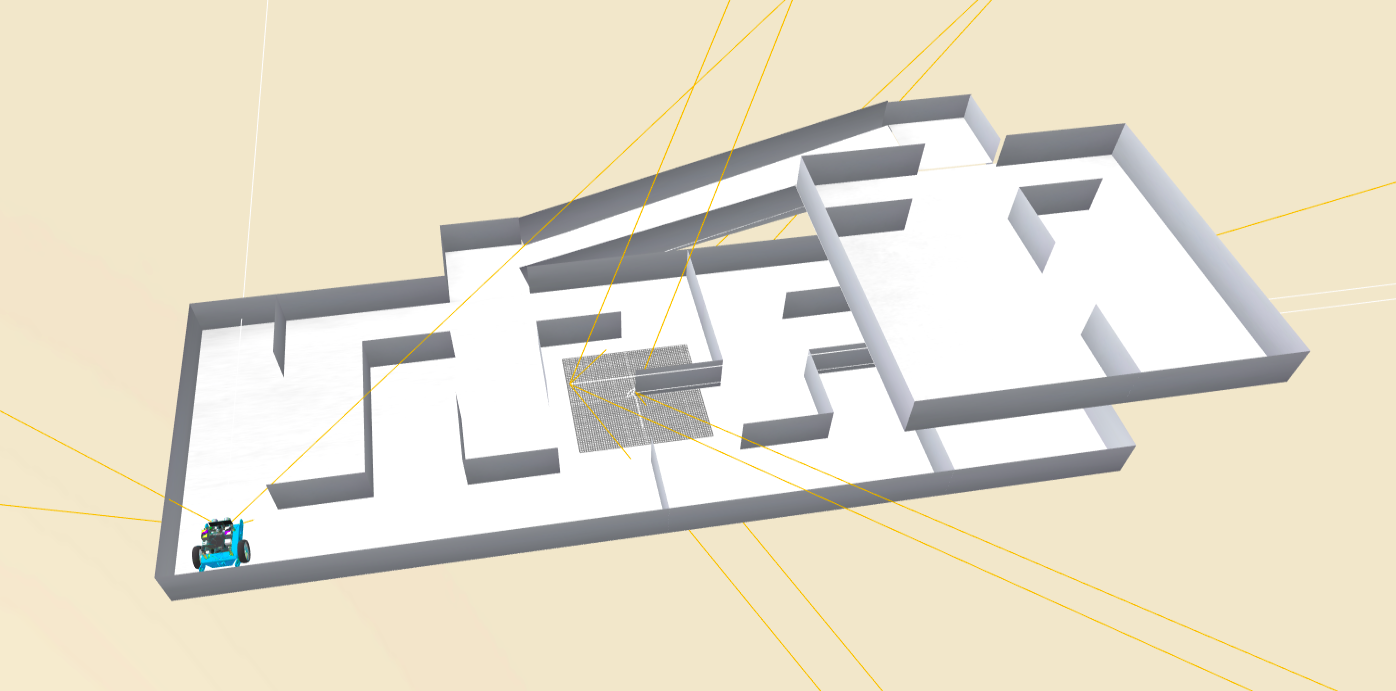
\includegraphics[width=0.8\textwidth, height=0.8\textwidth]{laberinto.png}
    \caption{Laberinto 3D para mBot}
    \label{fig:Laberinto 3D para mBot}
\end{figure}

\begin{figure}[h!]
\begin{subfigure}[b]{0.5\textwidth}
    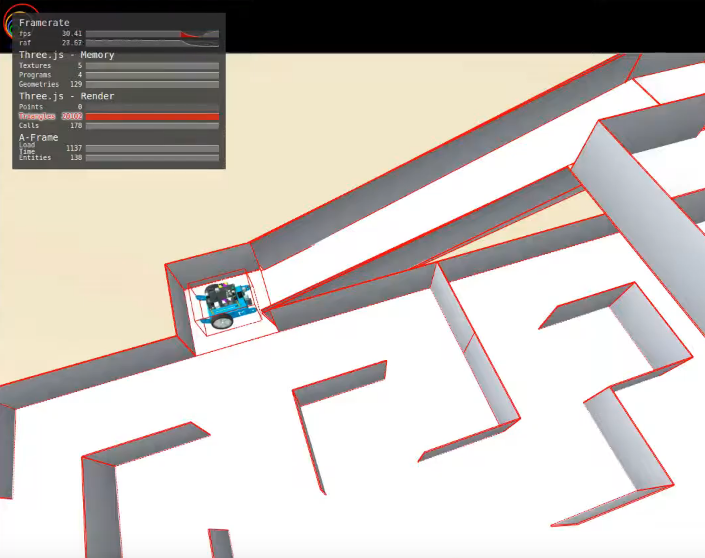
\includegraphics[width=\textwidth, height=\textwidth]{laberinto1.png}
  \end{subfigure}
  \hfill
  \hfill
  \begin{subfigure}[b]{0.5\textwidth}
    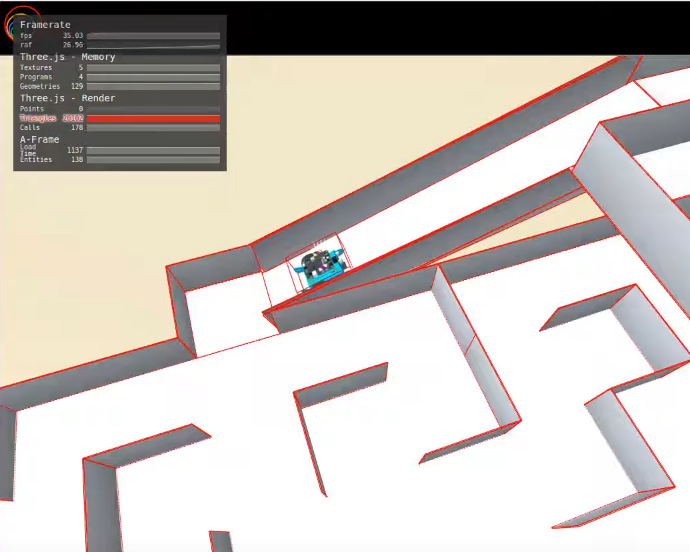
\includegraphics[width=\textwidth, height=\textwidth]{laberinto2.png}
  \end{subfigure}
    \hfill
    \hfill
  \begin{subfigure}[b]{0.5\textwidth}
    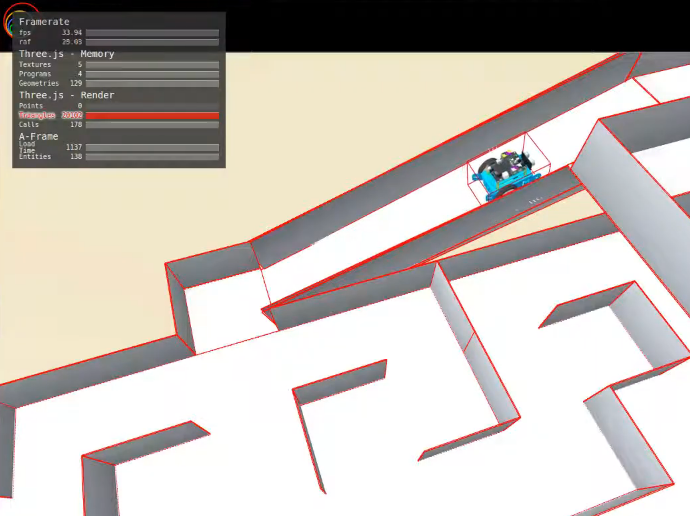
\includegraphics[width=\textwidth, height=\textwidth]{laberinto3ç.png}
  \end{subfigure}
    \hfill
  \begin{subfigure}[b]{0.5\textwidth}
    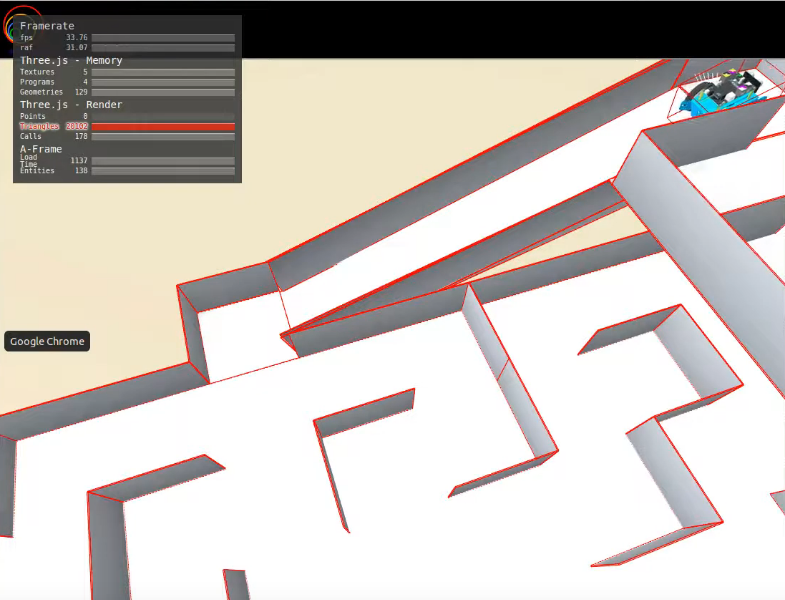
\includegraphics[width=\textwidth, height=\textwidth]{laberinto4.png}
  \end{subfigure}
    \caption{Fotograma del movimiento del ejercicio Laberinto 3D para mBot}
    \label{fig:laberinto_movimiento}
\end{figure}


\clearpage

A continuación, en la tabla \ref{tabla:param_ej2}, se recoge el valor de los parámetros del modelo de fuerzas y de  \textit{A-Frame} necesarios para el correcto funcionamiento del motor de físicas complementario y que caracterizan este ejercicio.

\begin{table}[h!]
\centering
\begin{tabular}{|c|c|}
\hline
\multicolumn{2}{|c|}{\textbf{Parámetros del modelo de fuerzas}}                \\ \hline
mass                                           & 1                             \\ \hline
inertia                                        & 1.3                           \\ \hline
Fmax                                           & 10                            \\ \hline
Tmax                                           & 1                             \\ \hline
accelerationMax                                & 10                            \\ \hline
angularAccelerationMax                         & 0.77                          \\ \hline
linealSpeedMax                                 & 10                            \\ \hline
angularSpeedMax                                & 5                             \\ \hline
\multicolumn{2}{|c|}{\textbf{Parámetros de \textit{A-Frame}}} \\ \hline
restitution                                    & 0.3                           \\ \hline
gravity                                        & -9.8                          \\ \hline
friction                                       &  0.0005                       \\ \hline
linearDamping                                  & -1.3                          \\ \hline
angularDamping                                 & -1.3                          \\ \hline
\end{tabular}
\caption{Parámetros de configuración del modelo de fuerzas y de \textit{A-Frame} del ejercicio laberinto 3D para mBot}
\label{tabla:param_ej2}
\end{table}

\newpage
\section{Laberinto para drone}
Se han incluido dos ejercicios nuevos para el drone Tello: laberinto para drone con y sin señalización. El objetivo de ambos ejercicios es que el drone encuentre la salida de un laberinto tridimensional. Este ejercicio aprovecha el motor de físicas complementario en el movimiento del drone, tanto durante el vuelo (controlador PD en velocidad) como cuando el drone permanece quieto a una cierta altura (controlador PD en posición)\footnote{\url{https://www.youtube.com/watch?v=jSGI6KJbzTQ}}. \newline

\begin{figure}[h!]
\begin{subfigure}[b]{0.3\textwidth}
    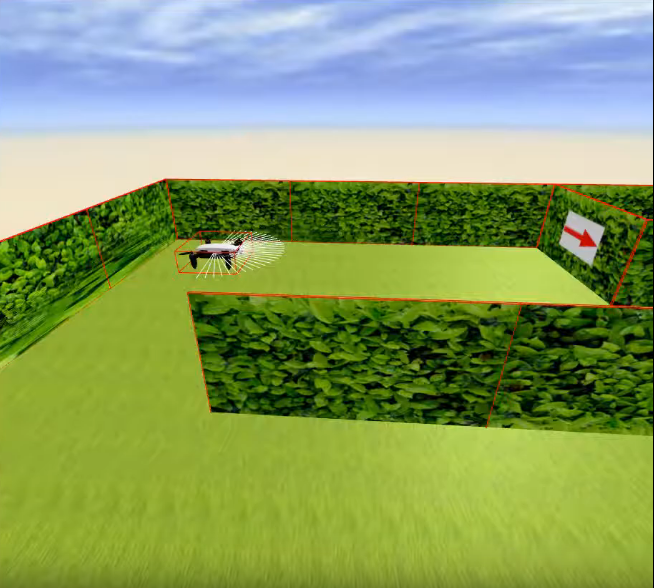
\includegraphics[width=\textwidth, height=\textwidth]{drone1.png}
  \end{subfigure}
  \hfill
  \hfill
  \begin{subfigure}[b]{0.3\textwidth}
    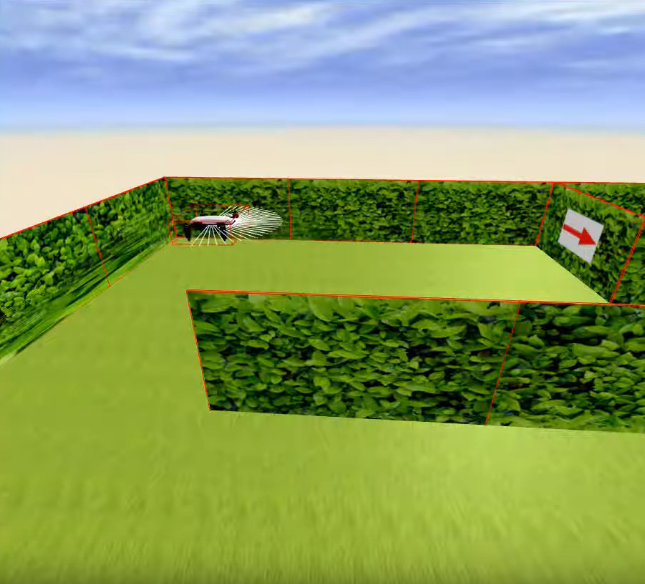
\includegraphics[width=\textwidth, height=\textwidth]{drone2.png}
  \end{subfigure}
    \hfill
    \hfill
  \begin{subfigure}[b]{0.3\textwidth}
    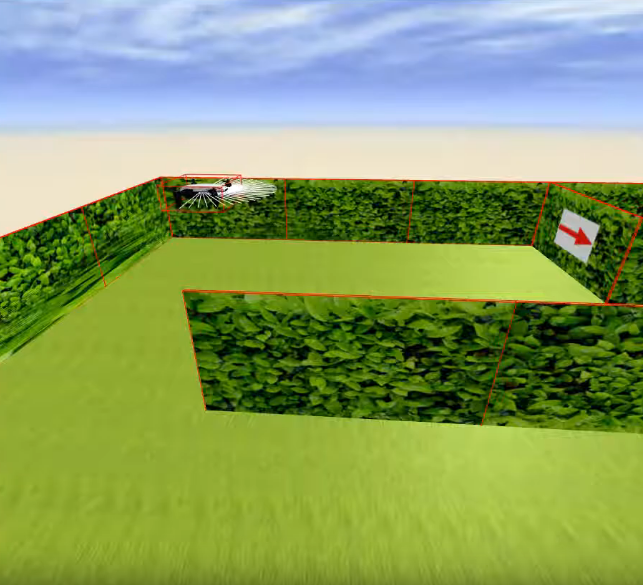
\includegraphics[width=\textwidth, height=\textwidth]{drone3.png}
  \end{subfigure}
    \hfill
    \caption{Fotograma del movimiento del ejercicio Laberinto para drone}
    \label{fig:laberinto_drone_movimiento}
\end{figure}

A continuación, en la tabla \ref{tabla:param_ej3}, se recoge el valor de los parámetros del modelo de fuerzas y de  \textit{A-Frame} necesarios para el correcto funcionamiento del motor de físicas complementario y que caracterizan este ejercicio.

\clearpage
\begin{table}[h!]
\centering
\begin{tabular}{|c|c|}
\hline
\multicolumn{2}{|c|}{\textbf{Parámetros del modelo de fuerzas}}                \\ \hline
mass                                           & 1                             \\ \hline
inertia                                        & 1.3                           \\ \hline
Fmax                                           & 10                            \\ \hline
Tmax                                           & 1                             \\ \hline
accelerationMax                                & 10                            \\ \hline
angularAccelerationMax                         & 0.77                          \\ \hline
linealSpeedMax                                 & 10                            \\ \hline
angularSpeedMax                                & 5                             \\ \hline
\multicolumn{2}{|c|}{\textbf{Parámetros de \textit{A-Frame}}} \\ \hline
restitution                                    & 0.3                           \\ \hline
gravity                                        & -9.8                          \\ \hline
friction                                       &  0.0000001                       \\ \hline
linearDamping                                  & 0.01                         \\ \hline
angularDamping                                 & 0.01                         \\ \hline
\end{tabular}
\caption{Parámetros de configuración del modelo de fuerzas y de \textit{A-Frame} del ejercicio laberinto para drone}
\label{tabla:param_ej3}
\end{table}

\subsection{Sin señalización}
La primera versión\footnote{\url{https://www.youtube.com/watch?v=RLjZPhP6P3g}} está pensada para que el usuario logre hacer que el drone encuentre la salida mendiante el uso de instrucciones en posición. Por ejemplo, 'avanza 2 metros' o 'gira a la derecha'.

\clearpage
\begin{figure}[h!]
    \centering
    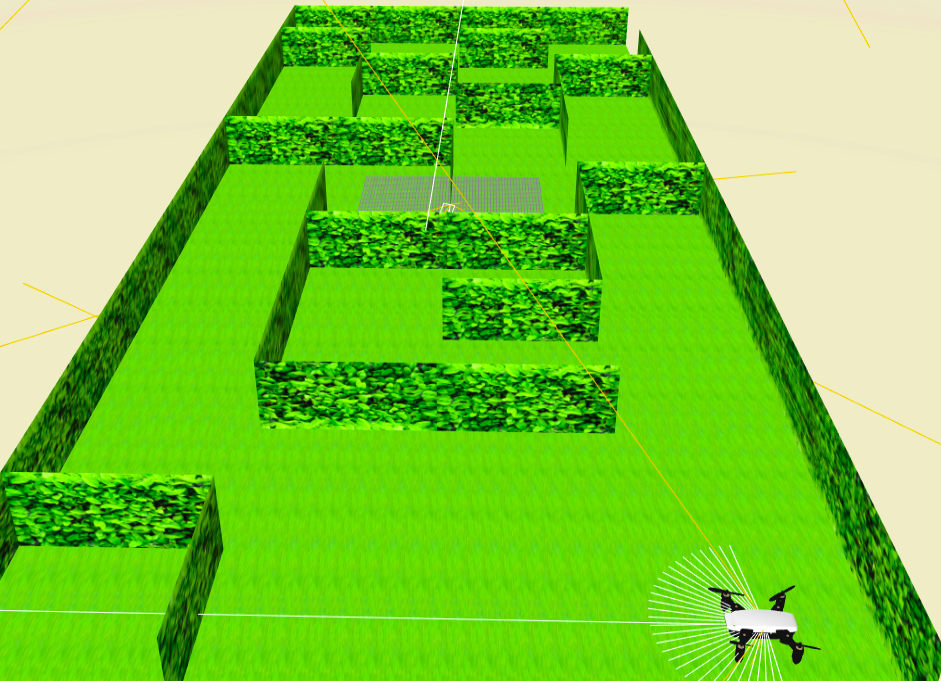
\includegraphics[width=0.8\textwidth, height=0.4\textwidth]{laberinto_drone.png}
    \caption{Laberinto para drone sin señalización}
    \label{fig:Laberinto_drone}
\end{figure}


\subsection{Con señalización}
La segunda versión\footnote{\url{https://www.youtube.com/watch?v=9tSqJQ7pqLc}} se ha implementado con el objetivo de que se utilicen los sensores y cámaras del drone para que se capten las señales que se han colocado por las paredes y que guían al drone para encontrar la salida. Gracias a la inteligencia artificial, el drone será capaz de reconocer las señales y traducirlas en un movimiento determinado.

\begin{figure}[h!]
    \centering
    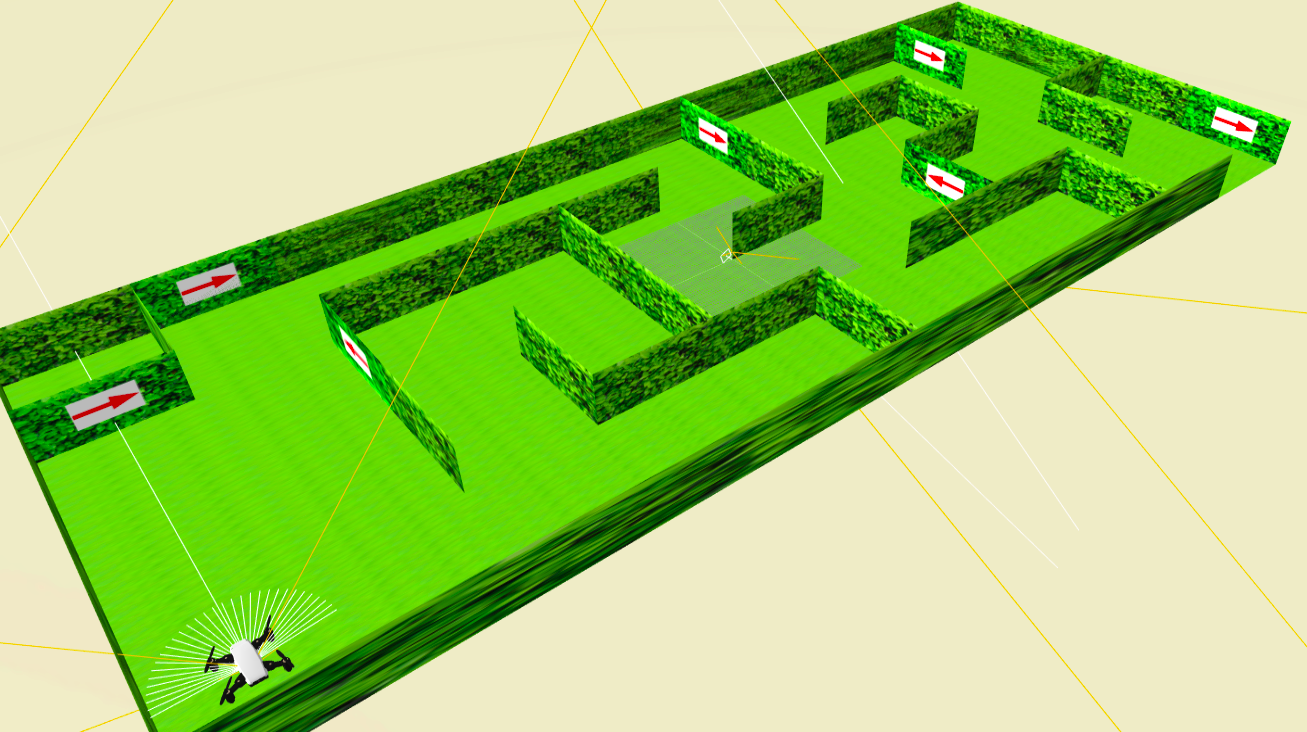
\includegraphics[width=0.8\textwidth, height=0.4\textwidth]{laberinto_drone_flecha.png}
    \caption{Laberinto para drone con señalización}
    \label{fig:Laberinto_drone_señal}
\end{figure}

\section{Fútbol competitivo}
Este último ejercicio\footnote{\url{https://www.youtube.com/watch?v=FYtAFll4keU}} también se basa en una de las propuestas presentadas para la competición \textit{Robocup Junior Australia 2019}\footnote{https://www.robocupjunior.org.au/}. El objetivo de este ejercicio competitivo es meter más goles que el contrincante, es decir, simular un partido de fútbol uno contra uno. El primero que llegue a diez goles, será el ganador. Para ello, se ha implementado un evaluador que lleva la cuenta de los goles metidos por cada equipo\footnote{https://www.youtube.com/watch?v=lgwECFpTgNk}(Figura \ref{fig:evaluador}). 

\begin{figure}[h!]
    \centering
    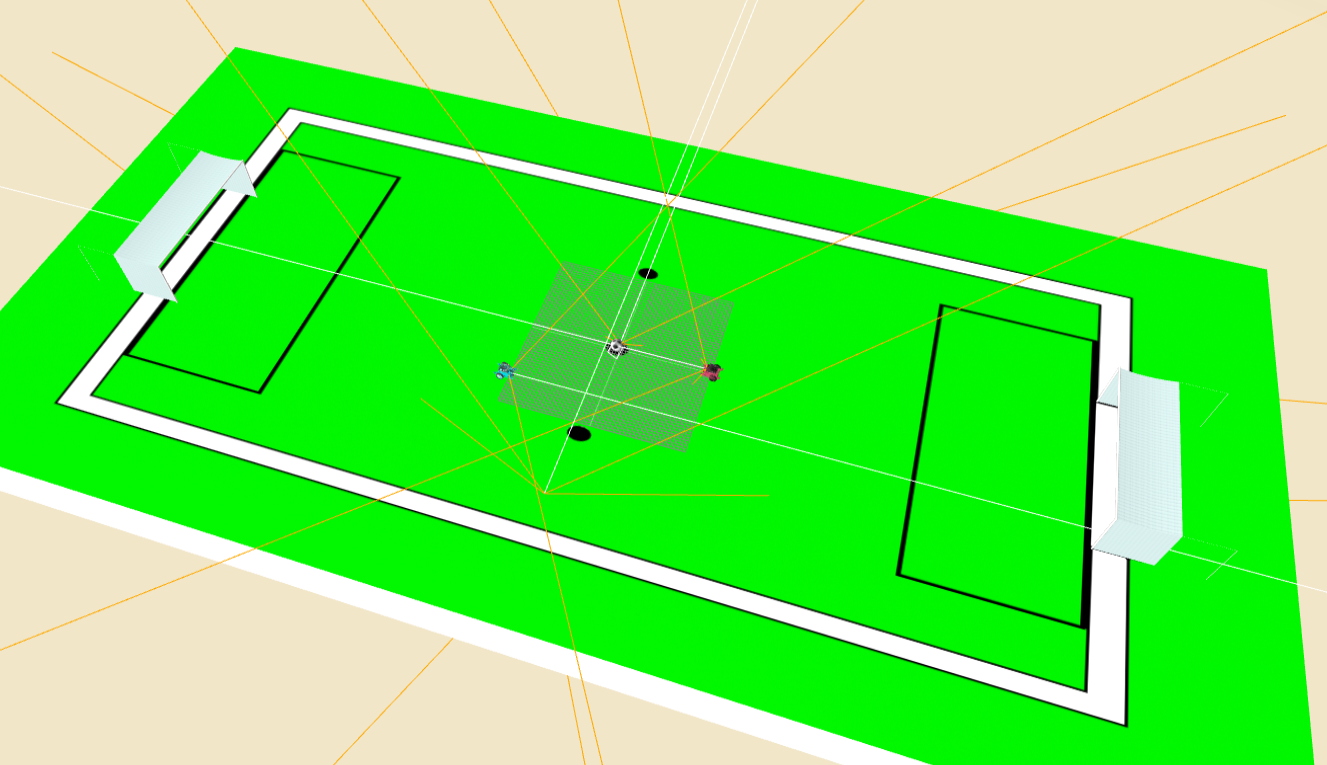
\includegraphics[width=\textwidth, height=0.8\textwidth]{poteria.png}
    \caption{Fútbol competitivo}
    \label{fig:futbol}
\end{figure}

\begin{figure}[h!]
  \begin{subfigure}[b]{0.5\textwidth}
    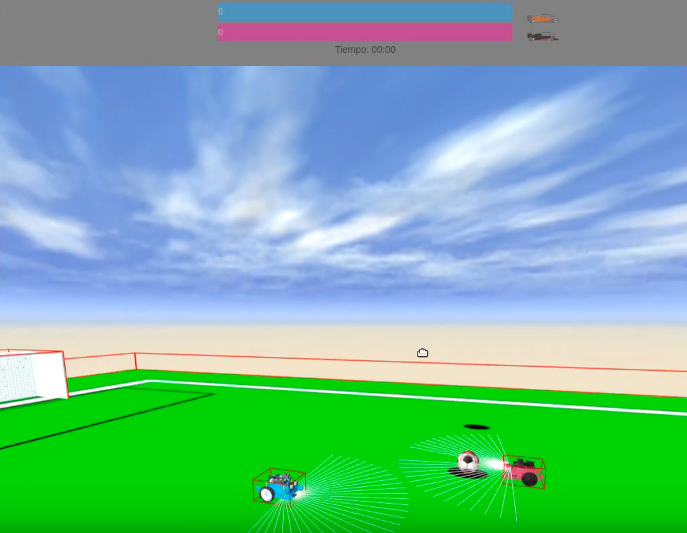
\includegraphics[width=\textwidth, height=\textwidth]{evaluador1.png}
  \end{subfigure}
  \hfill
  \hfill
  \begin{subfigure}[b]{0.5\textwidth}
    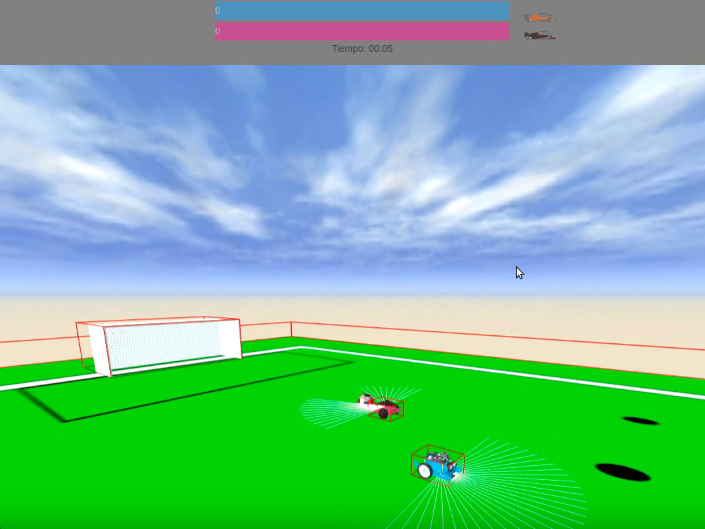
\includegraphics[width=\textwidth, height=\textwidth]{evaluador2.png}
  \end{subfigure}
    \hfill
    \hfill
  \begin{subfigure}[b]{0.5\textwidth}
    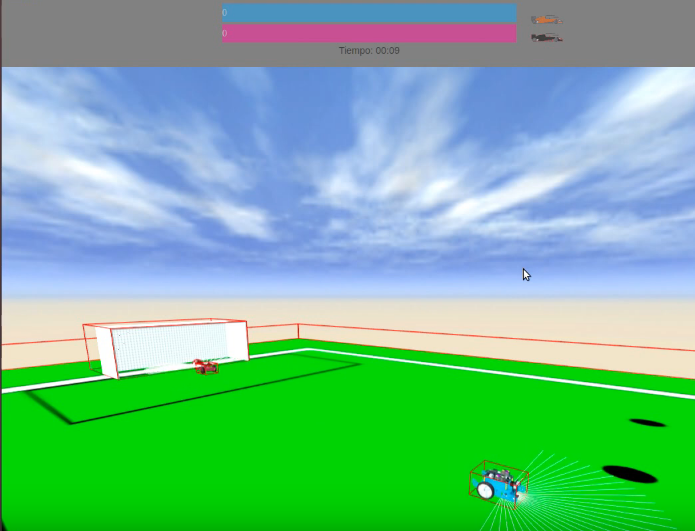
\includegraphics[width=\textwidth, height=\textwidth]{evaluador3.png}
  \end{subfigure}
    \hfill
  \begin{subfigure}[b]{0.5\textwidth}
    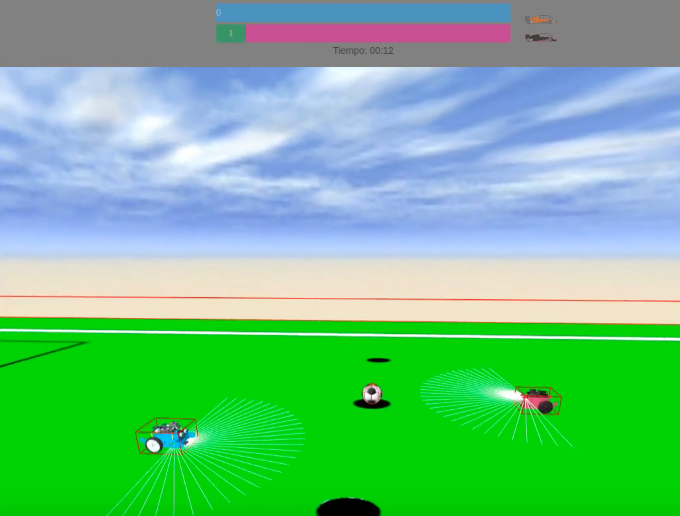
\includegraphics[width=\textwidth, height=\textwidth]{evaluador4.png}
  \end{subfigure}
\caption{Evaluador del ejercicio Fútbol competitivo}
\label{fig:evaluador}
\end{figure}

Este ejercicio saca provecho del estudio realizado en las físicas y del motor de físicas complementario tanto en los choques entre los robots y el balón como en el movimiento del balón. Ha sido necesaria la definición de un coeficiente de restitución adecuado para hacer realistas tanto los choques como el movimiento de la pelota. En este vídeo\footnote{\url{https://www.youtube.com/watch?v=7W-FB3E0B_I}} se observa un movimiento no realista del balón, mientras que en este otro\footnote{\url{https://www.youtube.com/watch?v=PIJRqBGPeH4}} se ha realizado el ajuste del coeficiente de restitución y la fricción, por lo que la pelota va girando sobre sí misma mientras va avanzando, haciendo mucho más realista el movimiento.

\clearpage

\begin{figure}[h!]
  \begin{subfigure}[b]{0.2\textwidth}
    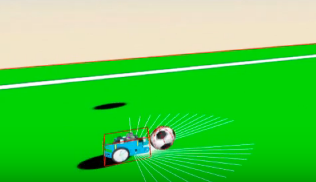
\includegraphics[width=\textwidth, height=\textwidth]{futbol1.png}
  \end{subfigure}
  \hfill
  \hfill
  \begin{subfigure}[b]{0.2\textwidth}
    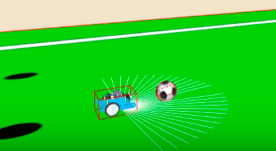
\includegraphics[width=\textwidth, height=\textwidth]{futbol2.png}
  \end{subfigure}
    \hfill
    \hfill
  \begin{subfigure}[b]{0.2\textwidth}
    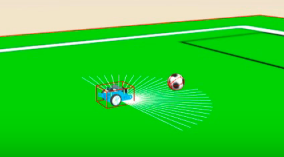
\includegraphics[width=\textwidth, height=\textwidth]{futbol3.png}
  \end{subfigure}
    \hfill
  \begin{subfigure}[b]{0.2\textwidth}
    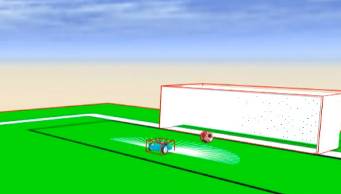
\includegraphics[width=\textwidth, height=\textwidth]{futbol4.png}
  \end{subfigure}
\caption{Fotograma del movimiento del ejercicio Fútbol competitivo}
\label{fig:movimiento_balón}
\end{figure}

A continuación, en la tabla \ref{tabla:param_ej4}, se recoge el valor de los parámetros del modelo de fuerzas y de  \textit{A-Frame} necesarios para el correcto funcionamiento del motor de físicas complementario y que caracterizan este ejercicio.

\begin{table}[h!]
\centering
\begin{tabular}{|c|c|}
\hline
\multicolumn{2}{|c|}{\textbf{Parámetros del modelo de fuerzas}}                \\ \hline
mass                                           & 1                             \\ \hline
inertia                                        & 1.3                           \\ \hline
Fmax                                           & 10                            \\ \hline
Tmax                                           & 1                             \\ \hline
accelerationMax                                & 10                            \\ \hline
angularAccelerationMax                         & 0.77                          \\ \hline
linealSpeedMax                                 & 10                            \\ \hline
angularSpeedMax                                & 5                             \\ \hline
\multicolumn{2}{|c|}{\textbf{Parámetros de \textit{A-Frame}}} \\ \hline
restitution                                    & 0.5                           \\ \hline
gravity                                        & -9.8                          \\ \hline
friction                                       &  0.0005                       \\ \hline
linearDamping                                  & 0.01                         \\ \hline
angularDamping                                 & 0.01                         \\ \hline
\end{tabular}
\caption{Parámetros de configuración del modelo de fuerzas y de \textit{A-Frame} del ejercicio fútbol competitivo}
\label{tabla:param_ej4}
\end{table}

